%%
% このファイルは、筑波大学情報学群情報メディア創成学類の
% 卒業研究論文本体のサンプルです。
% このファイルを書き換えて、この例と同じような書式の論文本体を
% LaTeXを使って作成することができます。
% 
% PC環境や、LaTeX環境の設定によっては漢字コードや改行コードを
% 変更する必要があります。
%%
\documentclass[a4paper,11pt]{jreport}

%%【PostScript, JPEG, PNG等の画像の貼り込み】
%% 利用するパッケージを選んでコメントアウトしてください。
%\usepackage{graphicx} % for 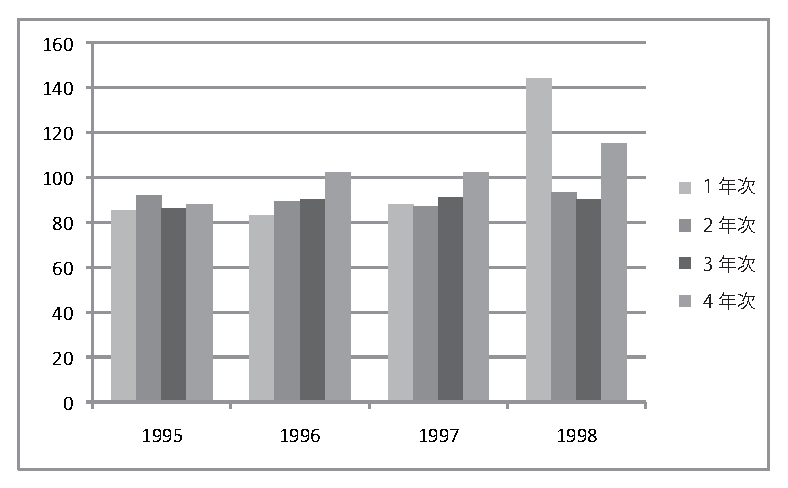
\includegraphics[width=3cm]{sample.eps}
\usepackage{epsfig} % for 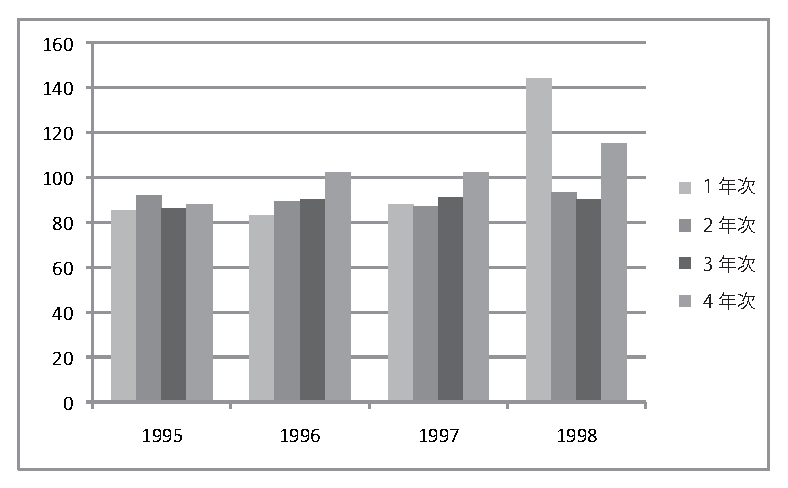
\psfig{file=sample.eps,width=3cm}
%\usepackage{epsf} % for \epsfile{file=sample.eps,scale=0.6}
%\usepackage{epsbox} % for \epsfile{file=sample.eps,scale=0.6}

\usepackage{times} % use Times Font instead of Computer Modern

%%%%%%%%%%追加
\usepackage{amsmath,amsthm,amssymb,cases}

\setcounter{tocdepth}{3}
\setcounter{page}{-1}

\setlength{\oddsidemargin}{0.1in}
\setlength{\evensidemargin}{0.1in} 
\setlength{\topmargin}{0in}
\setlength{\textwidth}{6in} 
%\setlength{\textheight}{10.1in}
\setlength{\parskip}{0em}
\setlength{\topsep}{0em}

%\newcommand{\zu}[1]{{\gt \bf 図\ref{#1}}}

%% タイトル生成用パッケージ(重要)
\usepackage{mast-jp-utf8}

%% タイトル
%% 【注意】タイトルの最後に\\ を入れるとエラーになります
\title{クエリ依存型リンク解析手法における\\スコア近似に関する研究}
%% 著者
\author{佐藤 豪}
%% 指導教員
\advisor{古瀬 一隆 陳 漢雄}

%% 年月 (提出年月)
%% 年月は必要に応じて書き替えてください。
\majorfield{ } \yearandmonth{2016年 1月}



\begin{document}
\maketitle
\thispagestyle{empty}
\newpage

\thispagestyle{empty}
\vspace*{20pt plus 1fil}
\parindent=1zw
\noindent
%%
%% 論文の概要(Abstract)
%%
\begin{center}
{\bf 概要}
\vspace{5mm}
\end{center}
私たちが普段使用しているWEBページの検索エンジンに用いられている手法の1つに、
リンク構造に基づいて得点を与えるSALSAアルゴリズムがある。
SALSAアルゴリズムはクエリ依存型のリンク解析手法であり、よりクエリに適した検索結果を得ることができる。一方で、クエリが与えられてからWEBグラフの抽出を行いリンク構造を取得し、各ページのスコア計算を行うため多くの応答時間がかかってしまう。

先行研究では、SALSAアルゴリズムの一部をクエリが与えられる前に処理することで高速化を図る手法が提案された。従来のSALSAアルゴリズムに比べて高速化することに成功したものの、ランキング精度においては著しく低い結果となり、クエリに適した検索結果が得られるというクエリ依存型リンク解析手法の長所が失われてしまった。そこで、本論文では先行研究の手法を改善し、ランキング精度を保ちつつ、高速化を行う手法を提案する。

本研究では、クエリ依存型リンク解析手法SALSAにおいて、クエリに適した検索結果が得られるという長所を保ちつつ、検索の高速化を行うことを目的とする。

%%%%%
\par
\vspace{0pt plus 1fil}
\newpage

\pagenumbering{roman} % I, II, III, IV 
\tableofcontents
\listoffigures
%\listoftables

\pagebreak \setcounter{page}{1}
\pagenumbering{arabic} % 1,2,3


%%%%%%%%%%%%%%%%%%%%%%%%%%%%%%%%%%%%%%%%%%%%%%%%
\chapter{序論}

世界中に10億件以上存在するWEBサイトの中から、必要な情報を手探りで探すことは困難である。
そのような場合、検索エンジンを用いることが有効である。検索エンジンは、ユーザーが必要とする情報に関連した検索キーワードを受け取り、そのキーワードに関連するWEBページの集合を抽出し、検索結果としてユーザーに掲示する。検索結果として掲示されるWEBページの集合は、検索キーワードとの関連度が高く、ユーザーにとって役に立つWEBページが上位に表示されることが望ましい。このように、ある検索ワードに関連するWEBページの集合に対して、ユーザーに掲示するための順位付けを行う手法をWEBランキングアルゴリズムと呼ぶ。

WEBランキングアルゴリズムは大きく分けて2種類ある。1つ目は、WEBページのテキストやHTML構造を解析することで内容得点を計算し、順位付けを行う手法である、2つ目は、WEBページ間のリンク構造に基づいてスコア計算を行い、順位付けを行うリンク解析手法である。本論文では後者のリンク解析手法を扱うものとする。

リンク解析手法のアルゴリズムで有名なものとしてPageRankアルゴリズムやHITSアルゴリズムが挙げられる。さらに近年の研究では、PageRankアルゴリズムとHITSアルゴリズムの長所を取り入れたSALSAアルゴリズムと呼ばれるリンク解析手法が、ランキング精度において他のWEBランキングアルゴリズムより優れているという報告がされている。

PageRankアルゴリズムは、検索キーワードに依存せずスコア計算を行い、順位付けをすることができる。このようなリンク解析手法をクエリ独立型と呼ぶ。一方でHITSアルゴリズムやSALSAアルゴリズムは、検索キーワードが与えられてからスコア計算と順位付けを行う。このようなリンク解析手法をクエリ依存型と呼ぶ。したがって、これらのアルゴリズムを検索エンジンで用いる場合、検索キーワードが与えられる前にスコア計算を行うPageRankアルゴリズムは高速に応答することができるのに対し、検索キーワードが与えられてからスコア計算を行うHITSアルゴリズムやSALSAアルゴリズムは応答時に無視できないほどの時間がかかってしまう。

この問題の解決策として、クエリ依存型リンク解析手法において時間のかかるスコア計算を前処理化することで、応答時間を減らすという手法が過去に提案された。これらの手法では、検索キーワードが与えられる前にあらかじめWEBページのクラスタリングを行い、クラスタ内での各ページのスコア計算を行う。検索キーワードが与えられた後は、そのクラスタとスコアを用いて結果を近似し、WEBランキングを作成する。しかし、これらの手法では近似したスコアと本来のSALSAアルゴリズムによるスコアが大きく異るため、応答時間は早くなるがランキング精度が下がる結果となった。

そこで本研究では、クエリ依存型リンク解析手法SALSAの前処理化におけるクラスタリングとスコア近似を改善することで、従来のSALSAアルゴリズムにより近いWEBランキングを作成することができ、かつ応答時間の少ない手法を提案する。



%%%%%%%%%%%%%%%%%%%%%%%%%%%%%%%%%%%%%%%%%%%%%%%%
\chapter{関連研究}

本章では、クエリ依存型リンク解析手法SALSAに関する技術について、特に関連のある研究について紹介する。

\section{WEBランキングアルゴリズムの歴史}

巨大化したWEBの中から目的のWEBページを見つけるには、検索エンジンを使うのが有効である。検索エンジンに与えた検索キーワード、別名クエリと関連のあるページに対して順位付けをするのがWEBランキングアルゴリズムである。

1998年までWEBランキングアルゴリズムは、WEBページのテキストやHTML構造といった内容得点で順位付けを行っていた。この内容得点というのは、各WEBページにどこにどれほどクエリの文字列が含まれているのか計算したものであった。しかし、WEBが巨大化し限りなく増大していったことや、内容得点がスパムの影響を受けやすかったことから、1998年までには従来の内容得点は有効でないことが明らかになっていた。

そこで、内容得点だけではなく、WEBのハイパーリンク構造に対して有向グラフを作成し、その有向グラフを用いてWEBページの人気得点を計算するリンク解析手法が登場した。これによって従来の内容得点によるランキングよりも品質が向上し、検索エンジンの利用者は劇的に増え、リンク解析手法はWEBランキングアルゴリズムの主流となった。


\begin{figure}[htbp]
\begin{center}
%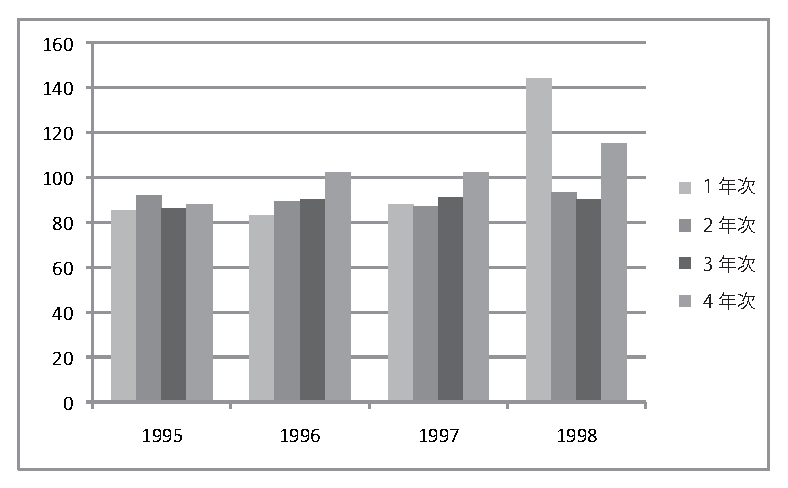
\includegraphics[width=3cm]{sample.eps}
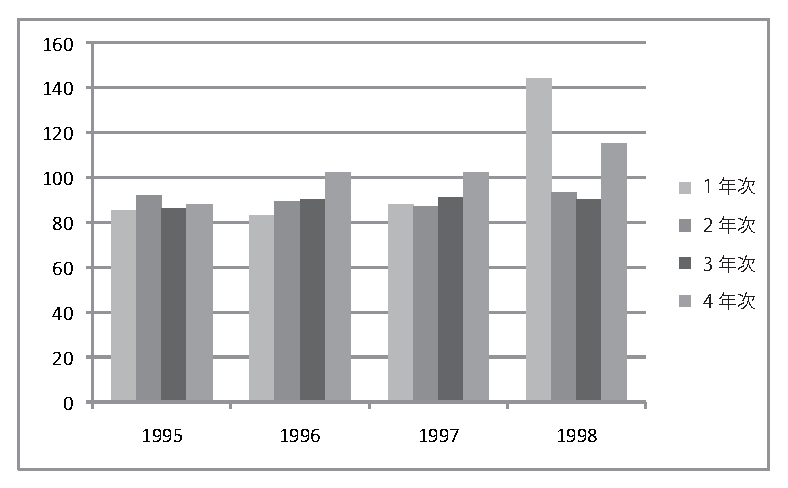
\psfig{file=sample.eps,scale=0.6}
%\epsfile{file=sample.eps,scale=0.6}
\end{center}
\caption{WEBグラフ}
\label{figure:sample}
\end{figure}


\section{PageRank}

PageRankは、当時Stanford Universityに在学していたSergey BrinとLarry Pageの2人の計算機科学科の学生によって開発されたものであり、開発者の名前がアルゴリズムの由来となっている。これがのちのWEB検索エンジンGoogleであり、このアルゴリズムの基本的な概念は「多くの良質なページからリンクされているページは、 やはり良質なページである」 という再帰的な関係をもとに、全てのページの重要度を判定したものである。

以下の図2.2はPageRankの概念図である。あるページのスコアを、そのページに存在する出リンク数で割った数が、それぞれの被リンク先のスコアに加算されるという関係になっている。

\begin{figure}[htbp]
\begin{center}
%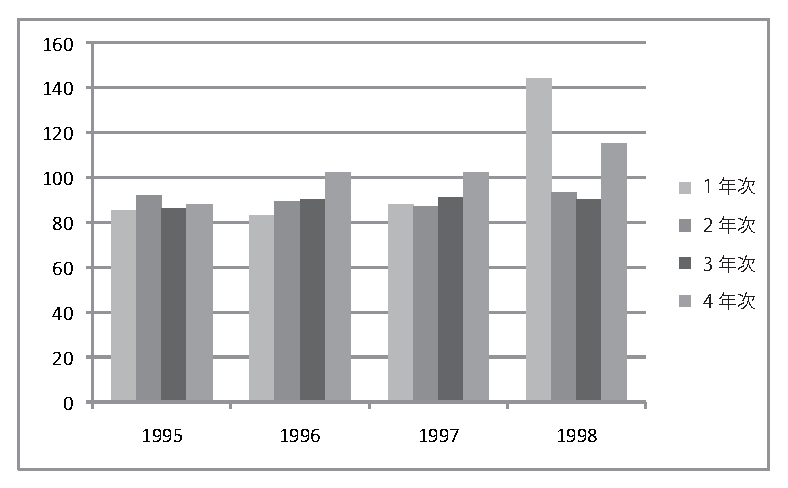
\includegraphics[width=3cm]{sample.eps}
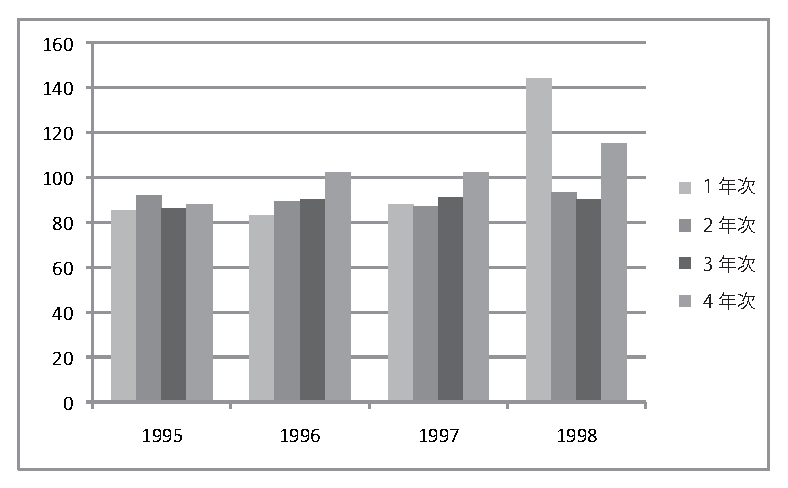
\psfig{file=sample.eps,scale=0.6}
%\epsfile{file=sample.eps,scale=0.6}
\end{center}
\caption{PageRankの概念図}
\label{figure:sample}
\end{figure}

PageRankは、WEBグラフにランダムウォークモデルを適応し、各ページヘの遷移確率によってWEBランキングを作成する。あるページからそのページが指している全リンク先へとランダムに遷移する確率と全てのWEBページへとランダムに遷移する確率を足したスコアがPageRankのスコアになる。

PageRankのスコア計算は以下の式(2.1)で定義される。

\begin{equation}
\pi^T = \pi^T(\alpha S + (1 - \alpha)E) 
\end{equation}

ここで$\pi^T$はPageRankベクトルであり、$\alpha$は0.85程度のスカラー値であり、行列$S$はページ$i$から
そのリンク先であるページ$j$への遷移確率行列である。また行列$E$は全てのWEBページヘのレポーテーション行列である。

ここで行列$S$は、ページ$i$からそのリンク先ページ$j$への遷移確率を示すので以下のように定義することができる。

\begin{equation}
S_(i,j) =
\begin{cases}
\; 1/out(i) (out(i)はノードiの出リンク数) \\
\; 0 (ノードiからノードjへのリンクがないとき)
\end{cases}
\end{equation}

また、行列$E$はページ$i$から全てのページへのランダムな遷移を示すので、以下(2.3)のように定義することができる。

\begin{equation}
E_(i,j) = 1
\end{equation}

PageRankの特徴の1つとして、クエリ独立型のリンク解析手法であるという点が挙げられる。
これは、クエリに関係なく、最初から全てのWEBページに対するWEBランキングが決定しているということである。クエリが与えられてからは、既に作成されているWEBランキングに適切なフィルタリングを施し、検索結果としてWEBランキングを表示するだけである。このためPageRankは、HITSやSALSAのようなクエリ依存型のリンク解析手法に比べ、応答時間が短い。

\section{HITS}
\section{SALSA}

%%%%%%%%%%%%%%%%%%%%%%%%%%%%%%%%%%%%%%%%%%%%%%%%
\chapter{提案手法}

てすてす

\section{クエリ依存型リンク解析手法高速化の概要}
\section{提案手法の概要}
\section{クラスタリングアルゴリズム}
\section{スコアの近似}

%%%%%%%%%%%%%%%%%%%%%%%%%%%%%%%%%%%%%%%%%%%%%%%%
\chapter{実験と考察}

てすてす

\section{評価指標}
\section{実データでの実験}
\section{大規模データでの実験}

%%%%%%%%%%%%%%%%%%%%%%%%%%%%%%%%%%%%%%%%%%%%%%%%
\chapter{まとめ}

てすてす

%%%%%%%%%%%%%%%%%%%%%%%%%%%%%%%%%%%%%%%%%%%%%%%%
\chapter{形式}

ここでは、論文の表紙および本体の記述方法について述べる。

\section{表紙}

表紙は、{\tt $\backslash$maketitle} によって作成するため、以下の項目に相
当する文字列をそれぞれ記述する。

\begin{description} \parskip=1pt
\item{題目: }
題目は{\tt $\backslash$title} に記述する。行替えを行う場合は$\backslash$
	   $\backslash$ を入力する。ただし、題目の最後に$\backslash$
	   $\backslash$ を入力するとコンパイルが通らなくなるので注意する。
	   なお、4行以上の題目の場合、表紙ページがあふれるためスタイルファ
	   イル``mast-jp-sjis.sty''を変更する必要がある。
\item{著者名: }
著者名は{\tt $\backslash$author} に記述する。
\item{指導教員名: }
指導教教員は{\tt $\backslash$advisor} に記述する。
\item{年月: }
年月は{\tt $\backslash$yearandmonth} に記述する。年月は提出時のものを記述すること。
\end{description}

\section{本体}

本体は1段組で記述する。

図表には番号と説明(caption)を付け、文章中で参照する。表
\ref{table:fundamental_data_type}と図\ref{figure:sample}はそれぞれ表と図
の例である。表の説明は上に、図の説明は下に書くことが多い。図の挿入に用い
るパッケージについては使用環境に合わせて自由に選択してほしい。

\begin{table}[hbt]
\caption{表の例}
\label{table:fundamental_data_type}
\begin{center}
\begin{tabular}{| c | r | r | r | r |}
\hline
年 度 & 1年次 & 2年次 & 3年次 & 4年次 \\
\hline
1995 & 85 & 92 & 86 & 88 \\
1996 & 83 & 89 & 90 & 102 \\
1997 & 88 & 87 & 91 & 112 \\
1998 & 144 & 93 & 90 & 115 \\
\hline 
\end{tabular}
\end{center}
\end{table}
\medskip

\begin{figure}[htbp]
\begin{center}
%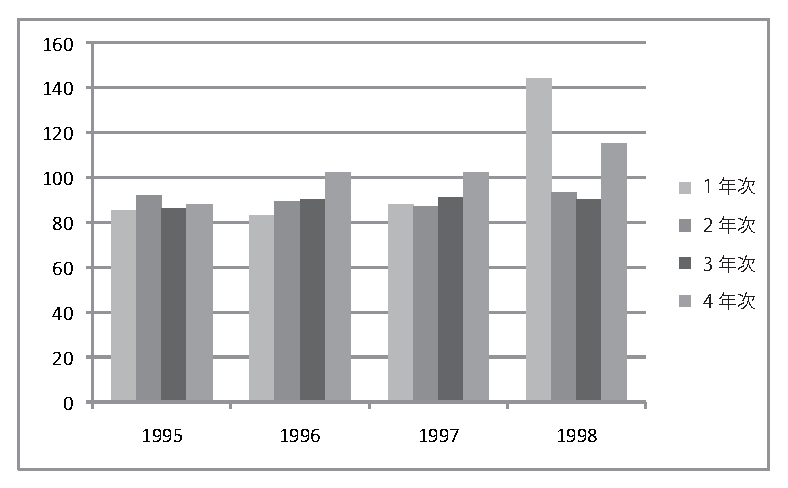
\includegraphics[width=3cm]{sample.eps}
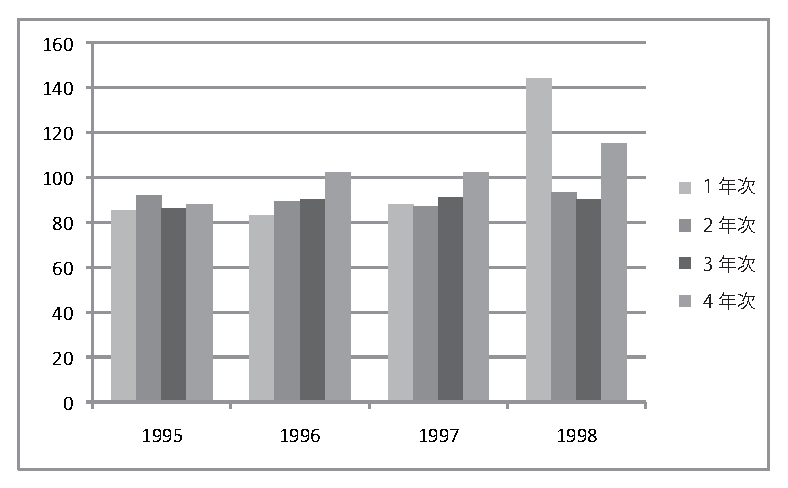
\psfig{file=sample.eps,scale=0.6}
%\epsfile{file=sample.eps,scale=0.6}
\end{center}
\caption{図の例}
\label{figure:sample}
\end{figure}

詳しくは参考書\cite{okumura2010,yoshinaga2009}などを参照のこと。
また、奥村晴彦氏の「\TeX Wiki」
http://oku.edu.mie-u.ac.jp/\textasciitilde{}okumura/texwiki/
は、日本語の\TeX に関する情報が充実している。
また、具体的な論文としての文献参照例として
(本の例)\cite{ware2004}、
(雑誌論文の例)\cite{meyer2009}、
(予稿集の例)\cite{hill2010}
を挙げておく。

\chapter*{謝辞}
\addcontentsline{toc}{chapter}{\numberline{}謝辞}

感謝

\newpage


\addcontentsline{toc}{chapter}{\numberline{}参考文献}
\renewcommand{\bibname}{参考文献}

%% 参考文献に jbibtex を使う場合
%\bibliographystyle{junsrt}
%\bibliography{samplebib}
%% [compile] jbibtex sample; platex sample; platex sample;

%% 参考文献を直接ファイルに含めて書く場合
\begin{thebibliography}{1}
\bibitem{okumura2010}
奥村晴彦, LaTeX2e美文書作成入門 改訂第5版, 技術評論社, 2010年.

\bibitem{yoshinaga2009}
吉永徹美, LaTeX2ε辞典, 翔泳社, 2009年.

\bibitem{ware2004} 
Colin Ware, Information Visualization --- Perception for Design, Second Edition, Morgan Kaufmann Publishers, 486~p., 2004.

\bibitem{meyer2009}
Miriah Meyer and Tamara Munzner, MizBee: A Multiscale Synteny Browser, {\em IEEE Transactions on Visualization and Computer Graphics}, Vol.~15, No.~6, pp.~897--904, 2009.

\bibitem{hill2010}
Emerson Murphy-Hill and Andrew P. Plack, An Interactive Ambient Visualization for Code Smells, {\em in Proceedings of the 2010 International Symposium on Software Visualization (SOFTVIS’10)}, pp.~5--14, 2010.

\end{thebibliography}




\end{document}
